\documentclass[a4paper]{IEEEtran}

\usepackage{xcolor}
\usepackage{hyperref}
\usepackage[utf8]{inputenc}
\usepackage[pdftex]{graphicx} 
\usepackage{multirow, pgfplotstable,booktabs,colortbl,lmodern}

\newcommand\TODO{\textcolor{red}{[TODO]}}
\newcommand\todo[1]{\textcolor{red}{[TODO: #1]}}
\newcommand\CN{\textcolor{blue}{[Citation Needed]}}
\newcommand\cn[1]{\textcolor{blue}{[Citation Needed: #1]}}

\title{The Cellular Automata Research Platform: PCIe}
\author{Per Thomas Lundal}

\begin{document}

\maketitle

\begin{abstract}

Lorem ipsum dolor sit amet, consectetur adipiscing elit. Vestibulum et nulla non dui mattis tincidunt. Vestibulum mattis volutpat tristique. Quisque sollicitudin ac eros et vulputate. Curabitur a libero ut diam cursus lobortis. Sed imperdiet, mauris a iaculis sodales, neque nisi consectetur libero, et vulputate lacus elit et nunc. Nunc at.

\end{abstract}

\section{Introduction}

\begin{itemize}
    \item What is a Cellular Automata?
    \item A little about FPGA and SBlocks.
    \item Motivation
\end{itemize}

\section{Related Work}

\begin{itemize}
    \item von Neumann's work on self-replication from around 1950 \cite{neumann1966selfreplication}.
    \item Turing-complete CA with 29 states
    \item Codd: Turing-complete CA with 8 states, given some conditions \cite{codd1968cellular}
    \item Langton's research on emergent computation and phase transition \cite{langton1990edgeofchaos}.
    \item Wolfram's quafitative CA classes \cite{wolfram1984complexity}?
\end{itemize}

\subsection{Evolution}

\begin{itemize}
    \item Genetic Algorithms
    \item Evolution in materio/silicon \cite{miller2014evolution}
\end{itemize}

\subsection{Artificial Development \cite{harding2008artificial}\cite{tufte2008evodevo}}
\begin{itemize}
    \item Zygote
    \item Scalability
    \item Robustness
    \item Plasticity
\end{itemize}

\section{Previous Work}

\subsection{Djupdal \cite{djupdal2003sblock}}

Fig. \ref{fig:ca-djupdal}

\begin{figure}[h!]
    \centering
    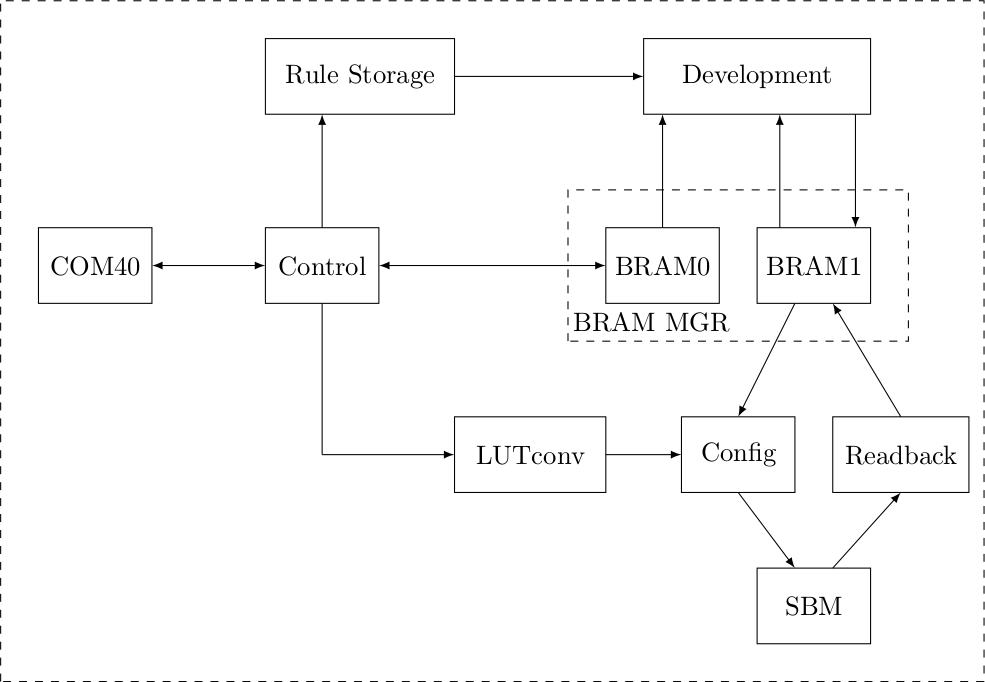
\includegraphics[width=0.5\textwidth]{figures/ca-djupdal}
    \caption{Original design by Djupdal (Reprinted from \cite{stovneng2014sblock})}
    \label{fig:ca-djupdal}
\end{figure}

\subsection{Aamodt \cite{aamodt2005sblock}}

Fig. \ref{fig:ca-aamodt}

\begin{figure}[h!]
    \centering
    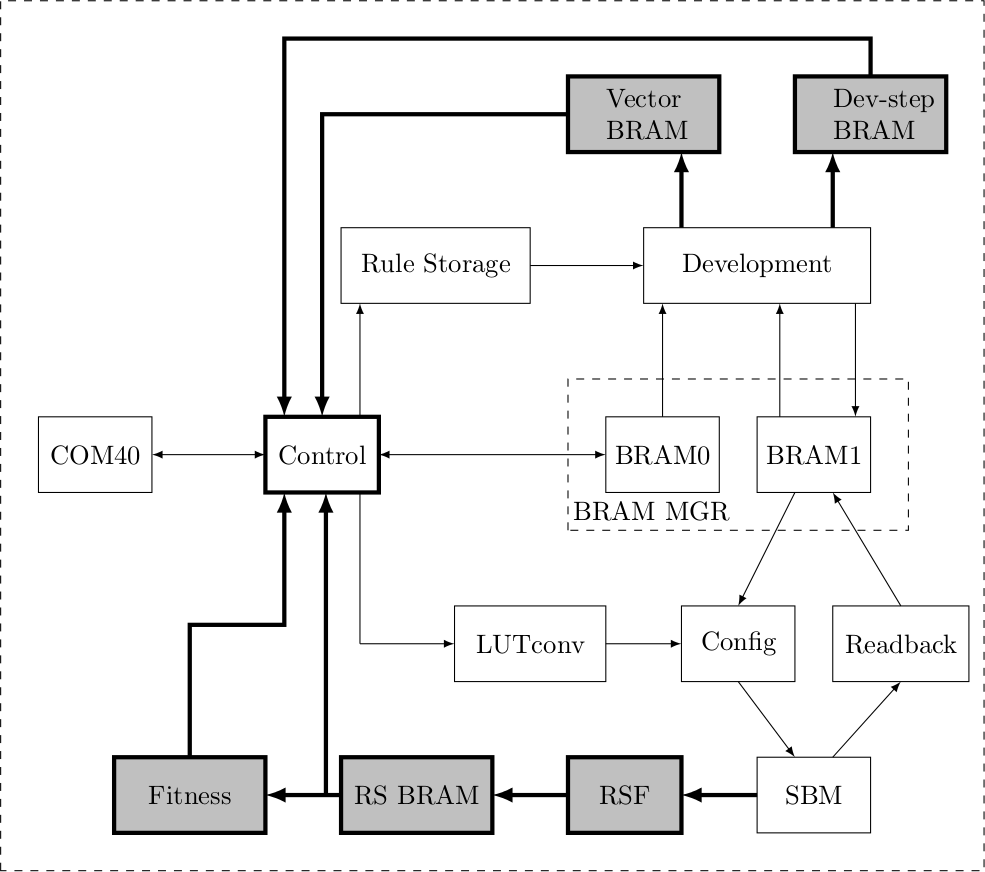
\includegraphics[width=0.5\textwidth]{figures/ca-aamodt}
    \caption{Additions by Aamodt (Reprinted from \cite{stovneng2014sblock})}
    \label{fig:ca-aamodt}
\end{figure}

\subsection{Støvneng \cite{stovneng2014sblock}}

Fig. \ref{fig:ca-stovneng}

\begin{figure}[h!]
    \centering
    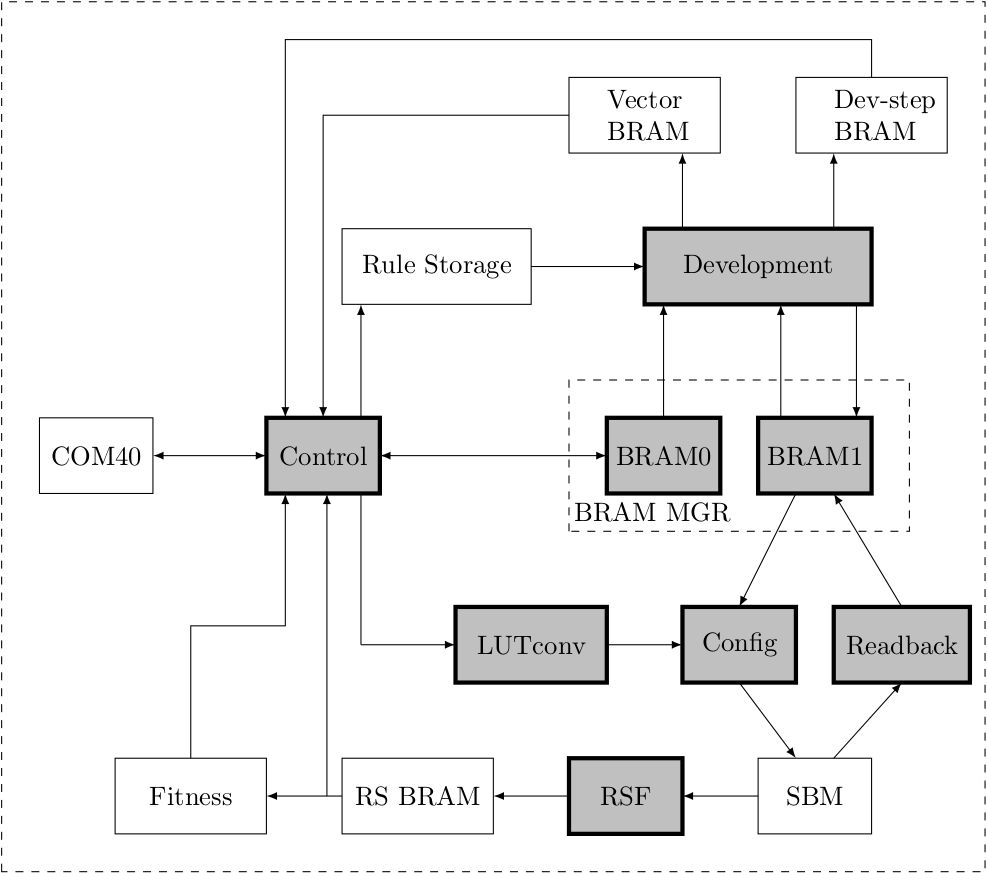
\includegraphics[width=0.5\textwidth]{figures/ca-stovneng}
    \caption{Parts optimized by Støvneng (Reprinted from \cite{stovneng2014sblock})}
    \label{fig:ca-stovneng}
\end{figure}

\todo{Tikz for diagrams: \url{http://www.texample.net/tikz/examples/noise-shaper/}}

\section{Methodology}

\TODO

\section{Results}

\TODO

\section{Discussion}

\TODO

\section{Conclusion}

\TODO

\bibliographystyle{IEEEtran}
\bibliography{IEEEabrv,bibliography}

\end{document}
